\chapter{Verarbeiten von Signalen}
\section{Durchf\"uhrung}
Die Aufgabe besteht nun darin, die Signale zu verarbeiten, was hier durch einfaches Verstärken oder Dämpfen realisiert wird.
In einem ersten Schritt wird das eingelesene Signal unverändert über den Codec zurückgegeben. Dies kann mittels \gls{vi} sichtbar gemacht werden. 
Dazu wurde der Funktionsgenerator auf \begin{math}V_{ss} = 1V\end{math} und 500Hz eingestellt, natürlich ergeben sich die üblichen Abweichungen von der tatsächlichen Messung.

\begin{figure}[h!]
  \centering
    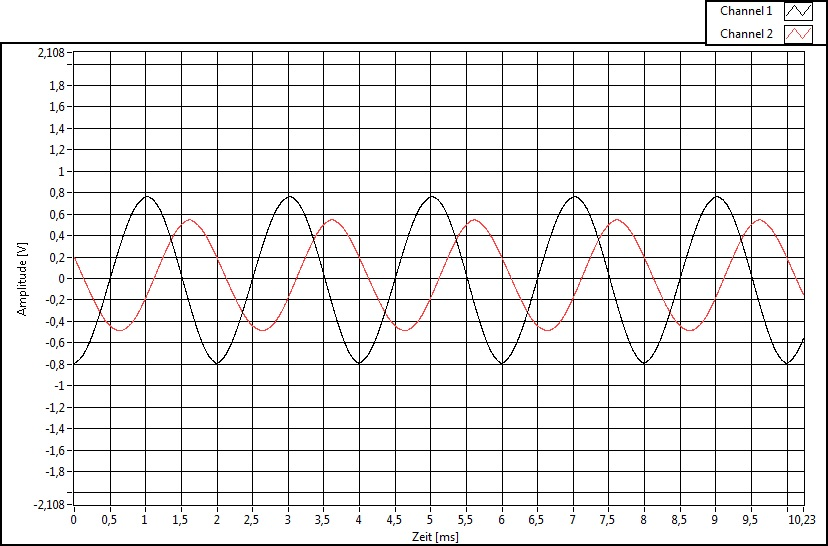
\includegraphics[width=\textwidth]{1V500Hz_ProgrammTest.jpg}
  \caption{Vergleich Eingang und Ausgang in C - 500Hz bei 1V}
  \label{fig:500HzC}
\end{figure}
\begin{figure}[h!]
  \centering
    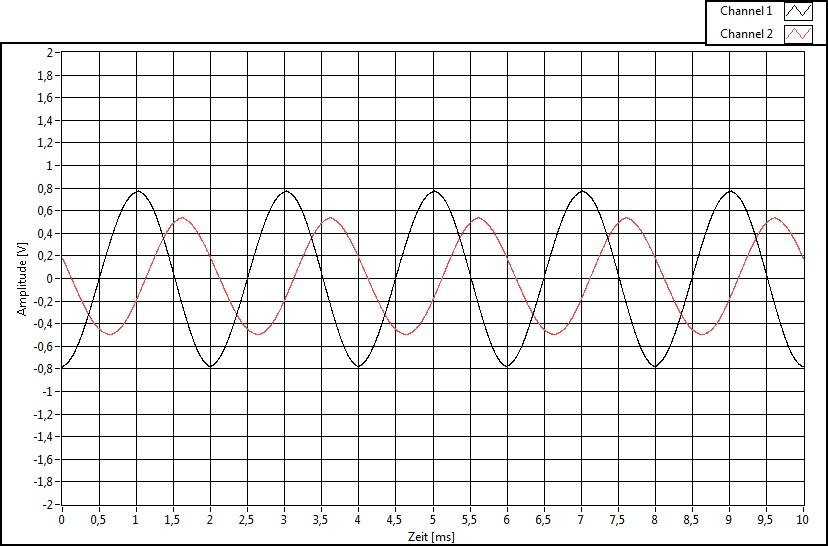
\includegraphics[width=\textwidth]{1V500Hz_AssemblerTest.jpg}
  \caption{Vergleich Eingang und Ausgang in Assembler - 500Hz bei 1V}
  \label{fig:500HzAss}
\end{figure}\pagebreak

Auch wurden die Frequenzgänge und Phasengänge mittels \gls{vi} visualisiert.

\begin{figure}[h!]
  \centering
    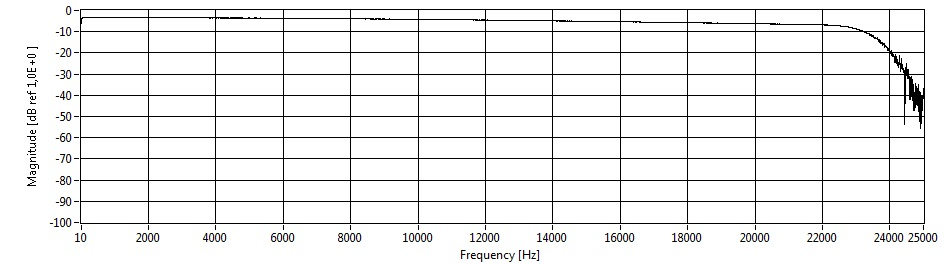
\includegraphics[width=\textwidth]{Frequenzgang_Gesamtsystem.jpg}
  \caption{Frequenzgang Gesamtsystem in C}
  \label{fig:FreqGGesC}
\end{figure}
\begin{figure}[h!]
  \centering
    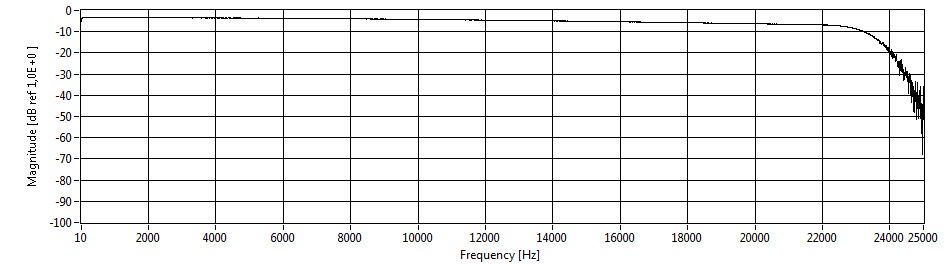
\includegraphics[width=\textwidth]{Frequenzgang_Gesamtsystem_asm.jpg}
  \caption{Frequenzgang Gesamtsystem in Assembler}
  \label{fig:FreqGGesAss}
\end{figure}
\begin{figure}[h!]
  \centering
    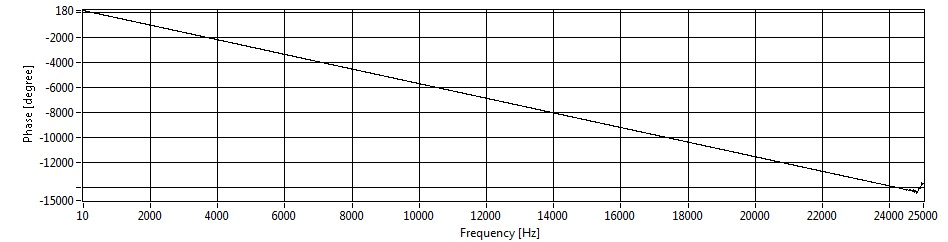
\includegraphics[width=\textwidth]{Phasengang_Gesamtsystem.jpg}
  \caption{Phasengang Gesamtsystem in C}
  \label{fig:PhaGGesC}
\end{figure}
\begin{figure}[h!]
  \centering
    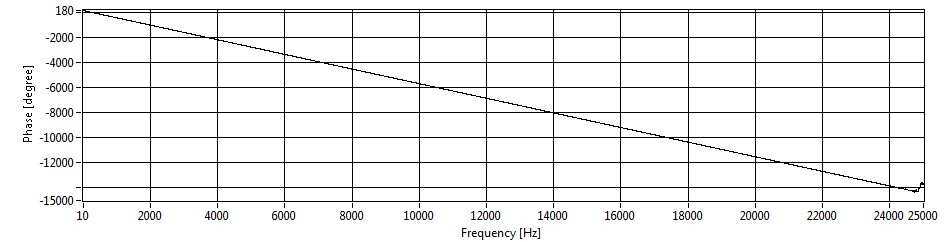
\includegraphics[width=\textwidth]{Phasengang_Gesamtsystem_asm.jpg}
  \caption{Phasengang Gesamtsystem in Assembler}
  \label{fig:PhaGGesAss}
\end{figure}

In Abbildung \ref{fig:500HzC} und Abbildung \ref{fig:500HzAss} ist kein Unterschied sichtbar. Dies entsprach den 
Erwartungen.\pagebreak

Wir haben die Umwandlung der ADC-Werte vom Hexadezimalen in das Signed Integer Format überprüft indem wir im Debugmodus das Programm anhielten und uns die Werte notierten.

\begin{center}
    \begin{tabular}{ | l | l | }\hline
      \multicolumn{2}{|c|}{iADC2R}\\
    \hline
    Hexadezimal & Dezimal \\ \hline
    00d2d300 &	13.881.856,00 \\ \hline
    0038d700 &	14.104.576,00 \\ \hline
    0047d600 &	14.042.880,00 \\ \hline
    00e4d300 &	13.886.464,00 \\ 
    \hline
    \end{tabular}
\end{center}
Es ist zu erkennen, dass das niederwertige Byte stets mit 00h gefüllt ist, 
dies begründet sich darin, dass die 24-bit des Codec stets in die höherwertigen Stellen geschrieben werden.

Im nächsten Schritt wurde das Programm in Assembler auf 16-bit umgestellt, da dies der optimierte Arbeitsbereich des DSP ist.
Hierzu wurde die isr.asm zur isr\textunderscore s.asm mit folgender Änderung entsprechend der 
Aufgabenstellung:\\
 \begin{lstlisting}[title=isr\textunderscore s.asm]{isr_s.asm}
        P1.L = _iDMARxBuffer; 
        P1.H = _iDMARxBuffer;

        R1 = [P1+INTERNAL_ADC_L1*4];
        P2.L = _sADC2L; P2.H = _sADC2L;
        W[P2] = R1.H;//W hinzugefügt um nur die oberen 16-bit zu wählen.
        
        R2 = [P1+INTERNAL_ADC_R1*4];
        P2.L = _sADC2R; P2.H = _sADC2R;
        W[P2] = R2.H;//W hinzugefügt um nur die oberen 16-bit zu wählen.

        P1.L = _iDMATxBuffer; 
        P1.H = _iDMATxBuffer;

        P2.L = _sDAC1L; P2.H = _sDAC1L;
        R1.H = W[P2];//W hinzugefügt um nur die oberen 16-bit zu wählen.
        [P1+INTERNAL_DAC_L0*4] = R1;
        
        P2.L = _sDAC1R; P2.H = _sDAC1R;
        R1.H = W[P2];//W hinzugefügt um nur die oberen 16-bit zu wählen.
        [P1+INTERNAL_DAC_R0*4] = R1;
 \end{lstlisting}

Ein entsprechender Test zeigt, dass keine Veränderung sichtbar wurde.
\begin{figure}[h!]
  \centering
    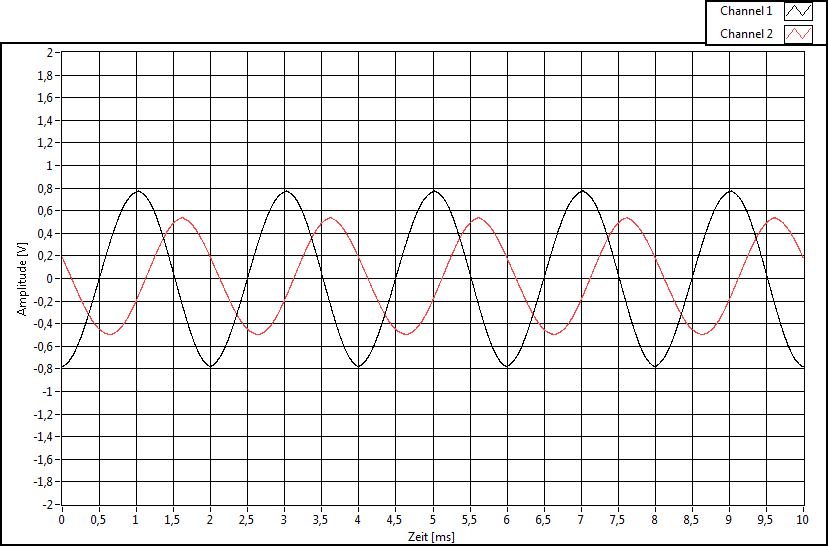
\includegraphics[width=\textwidth]{1V500Hz_AssemblerTest_16Bit.jpg}
  \caption{Vergleich Eingang und Ausgang in C und 16-bit - 500Hz bei 1V}
  \label{fig:500HzC16}
\end{figure}
  
\pagebreak



Der letzte Abschnitt der Aufgabe beinhaltete eine Amplitudenver\"anderung des Signals. Dies wurde in process\textunderscore data\textunderscore s.asm 
bearbeitet.\\
\lstinputlisting[title=processdatas.asm]{processdatas.asm}
Für die einzelnen Tests wurden die entsprechenden Zeilen die nicht genutzt wurden kommentiert. So ist in diesem Beispiel die Variante der Arithmetischen Division durch vier zu sehen.
\section{Auswertung}
In den folgenden Bildern ist das Originalsignal in schwarz und das \gls{evb}-Ausgangssignal mit Verzögerung und Amplitudenver\"anderung zu 
erkennen.\pagebreak

\begin{figure}[h!]
  \centering
    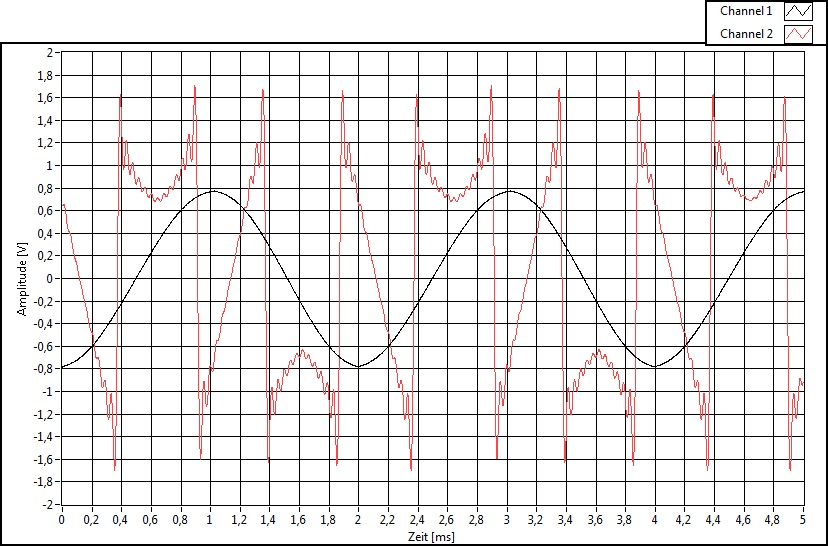
\includegraphics[width=\textwidth]{Mul4_ohneS.jpg}
  \caption{Multiplikation mit 4 ohne Sättigung}
  \label{fig:Mul4_ohneS}
\end{figure}
In Abbildung \ref{fig:Mul4_ohneS} ist ein \"Uberlaufverhalten zu erkennen, welches zu entsprechenden Fehlern führt. Außerdem ist dem Signal ein Rauschen 
überlagert.

\begin{figure}[h!]
  \centering
    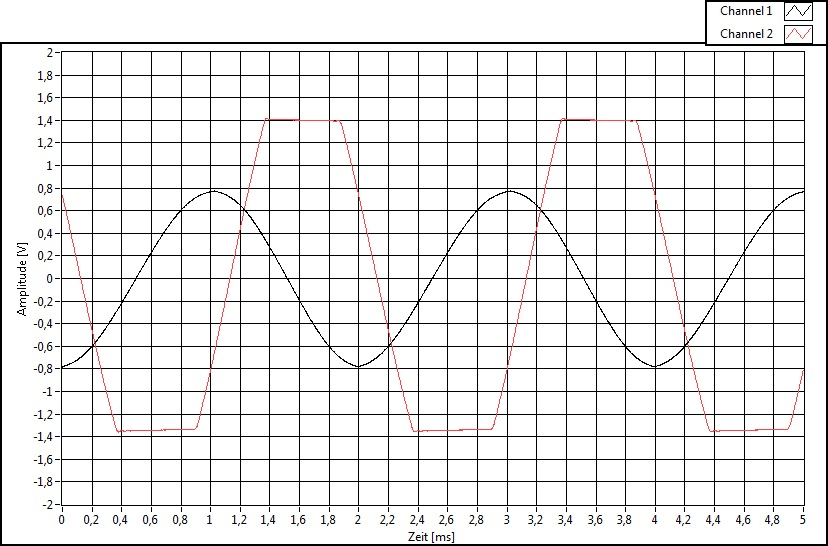
\includegraphics[width=\textwidth]{Mul4_mitS.jpg}
  \caption{Multiplikation mit 4 mit Sättigung}
  \label{fig:Mul4_mitS}
\end{figure}

Im Unterschied zur Abbildung \ref{fig:Mul4_ohneS} ist in Abbildung \ref{fig:Mul4_mitS} zu sehen, dass es zu keinen reinen Überläufen kommt, sondern der maximale Aussteuerungsbereich verwendet wird.
Dies führt zu geringeren Fehlern, allerdings ist der originale Signalverlauf nicht rekonstruierbar, da die Maxima nicht mehr sichtbar sind.
\begin{figure}[b!]
  \centering
    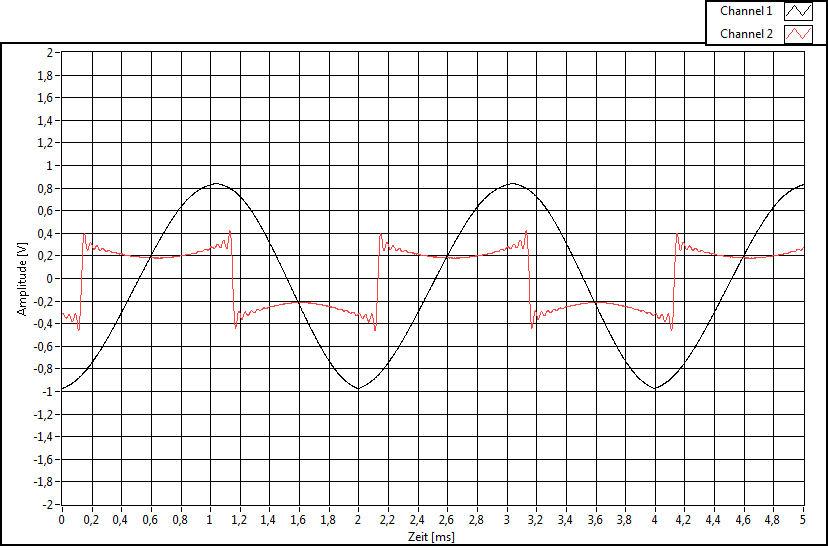
\includegraphics[width=\textwidth]{divlog.png}
  \caption{Logische Division mit 4}
  \label{fig:divlog}
\end{figure}
Der  logische  Shift  sorgt  f\"ur  den  Verlust  des  Vorzeichens,  was  zu  rein  positiven  Werten
f\"uhrt, da immer eine 0 nachgeschoben wird. 
Es sind nicht nur positive Werte zu sehen, da dieser Gleichanteil durch die Gleichspanungsentkopplung des Codes gefiltert wird.
Die Verringerung der Amplitude ist trotzdem zu sehen. 
Der arithmetische Shift verändert das Vorzeichen des Signals nicht und ermöglicht es den Signalverlauf beizubehalten. 
Lediglich die \"Anderung der Amplitude macht sich bemerkbar.
\begin{figure}[h!]
  \centering
    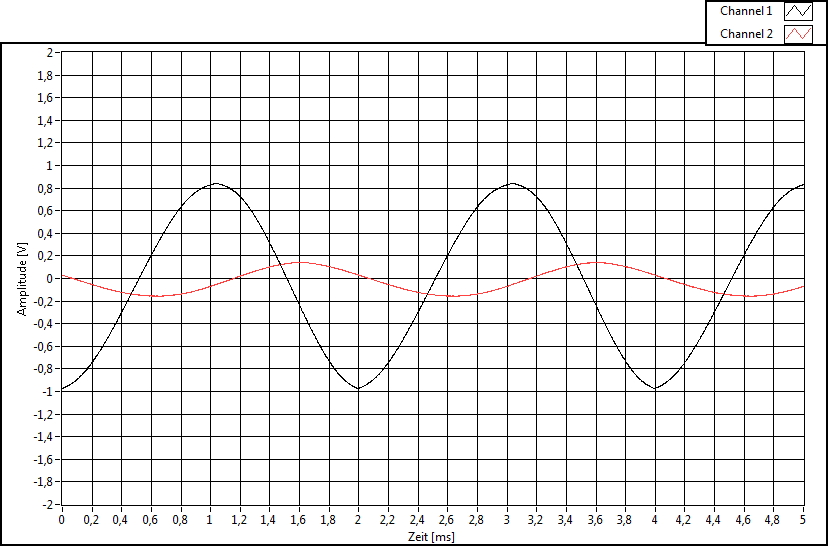
\includegraphics[width=\textwidth]{divarith.png}
  \caption{Arithmetische Division mit 4}
  \label{fig:divarith}
\end{figure}

Der arithmetische Shift behält stets sein Vorzeichen und ermöglicht daher das Signal beizubehalten und lediglich die \"Anderung der Amplitude macht sich 
bemerkbar.\\\par \pagebreak
Die Signallaufzeit lässt sich mit Hilfe des Phasenganges Graphisch ermitteln. 
In Abbildung \ref{fig:PhaGGesAss} und Abbildung \ref{fig:PhaGGesC} ist eine Phasenverschiebung -8000° bei 14kHz zu erkennen. Dies entspricht etwa 22 
Perioden.\\\par
Gemäß \begin{math}\frac{22}{14kHz} = 1,6ms\end{math} ergibt sich eine Laufzeit von 1,6ms. 
Diese Zeit resultiert zum einen aus der Verarbeitung durch die Software, aber auch durch die Wandlungen des Codec, wobei die Wandlungen den größten Anteil haben dürften. 
Ein weiterer Teil der Verzögerung wird dadurch verursacht, dass zwischen Ermitteln der Werte des ADC und Ablegen dieser im Speicher ein Taktzyklus liegt.

%Bitte alle code dateien die wir bearbeitet ahben anhängen
